\section{Why Transfer Displacements?}
\label{sec:supp_displacement}

TIE preserves a missing grade's own reference and supplies adaptation from its seen neighbors.
We separate these two choices, compare the inheritance rules, and identify the component of inheritance error that can change ranking.

\subsection{What to Keep, What to Inherit}
\label{sec:supp_keep_inherit}

Write the adapted scores as $S=T+D$ and suppress the image argument when it is not needed.
Let $\bar T_m$ and $\bar D_m$ denote the reference and displacement inherited from the same seen anchors with the same weights.
TIE uses equal weights for two bracketing anchors and copies the sole anchor when only one side is available.
Table~\ref{tab:supp_constructions} separates preserving the missing grade's reference from supplying its displacement.
All four constructions leave seen-grade scores at $S_n$.
The numerical comparison in Table~\ref{tab:supp_operator_comparison} uses the same scores and test images for every construction.

\begin{table}[t]
\centering
\caption{\textbf{What is preserved and what is inherited.}
Score constructions for a missing grade $m$.
The two inherited terms use the same anchors and weights; equal weights give TIE.
Seen-grade scores remain adapted.}
\label{tab:supp_constructions}
\small
\setlength{\tabcolsep}{4pt}
\begin{tabular*}{\columnwidth}{@{}l@{\extracolsep{\fill}}cc@{}}
\toprule
Construction & Reference & Displacement \\
\midrule
Adapted & $T_m$ & $D_m$ \\
Reference-only & $T_m$ & $0$ \\
TIE & $T_m$ & $\bar D_m$ \\
Direct score interpolation & $\bar T_m$ & $\bar D_m$ \\
\bottomrule
\end{tabular*}
\end{table}

\noindent\textbf{Preserving the reference.}
At identical weights, displacement transfer and direct score interpolation differ by exactly $T_m-\bar T_m$.
Direct score interpolation replaces the missing grade's own reference with its neighbors' reference.
At an endpoint with seen anchor $n$, it copies $S_n$, making the $m$--$n$ margin zero for every image.
All comparisons tie, so pair AUROC is exactly $0.5$.
TIE instead preserves the zero-shot margin $T_m-T_n$.
This distinction gives the missing grade its own image-dependent evidence even when it shares an adapted displacement with a neighbor.

\noindent\textbf{Supplying adaptation.}
Reference-only sets $D_m=0$ while retaining adaptation at the seen grades.
Its margin against a seen grade is
\begin{equation}
g^{\mathrm{ref}}_{mn}
=T_m-(T_n+D_n)
=g^T_{mn}-D_n.
\label{eq:supp_reference_only}
\end{equation}
Returning one score to zero-shot therefore does not restore the zero-shot pair margin.
The seen grade still carries its image-dependent displacement.
At an endpoint, TIE removes this asymmetry by sharing $D_n$ while preserving $T_m$.
Setting the missing-grade displacement to zero lowers MS-AUC on all four datasets, despite reducing Missing MAE (Table~\ref{tab:supp_operator_comparison}).
TIE achieves higher MS-AUC and lower Missing MAE than both Reference-only and direct score interpolation on every dataset.
These controls show why TIE combines the grade's own reference with its neighbors' displacement.

\subsection{Neighbor Selection and Inheritance Weights}
\label{sec:supp_inheritance_rules}

For an interior missing grade $m$, let $\ell<m<r$ be its nearest seen anchors.
Left- and right-anchor inheritance use $D_\ell$ and $D_r$, respectively, when both anchors are available.
TIE uses their mean.
Distance-weighted inheritance uses $\bar D_m^{\mathrm{dist}}=(1-\alpha_m)D_\ell+\alpha_mD_r$, where $\alpha_m=(m-\ell)/(r-\ell)$ is measured in grade indices.
When only one anchor is available, each inheritance rule copies it.
For an isolated interior grade, $\ell=m-1$ and $r=m+1$, so distance weights and equal weights coincide.
They differ within missing blocks.

One-sided inheritance exactly restores the zero-shot margin against its chosen anchor.
Two-sided inheritance additionally retains the contrast between the anchors: against the left anchor, $g^{\mathrm{TIE}}_{m\ell}=g^T_{m\ell}+\tfrac12(D_r-D_\ell)$.
Table~\ref{tab:supp_operator_comparison} compares these rules using the same scores, masks, and test images.
The choice of anchor matters: right-anchor inheritance is strongest on Adience, whereas TIE achieves higher MS-AUC than either one-sided rule on FairFace and KonIQ.
Distance weighting remains close to equal weights in the all-mask average, while the block analysis reveals where they differ.
MS-AUC measures the ranking effect; Missing MAE reports the resulting decisions before calibration.

\begin{table*}[t]
\centering
\caption{\textbf{Isolating the reference, displacement, and anchor rule.}
All constructions use the same zero-shot and adapted scores and leave seen-grade scores unchanged.
Each dataset averages nine adapter configurations equally, with six masks and three seeds per configuration (162 conditions).
MS-AUC $\uparrow$ measures missing--seen ranking; MAE $\downarrow$ is the macro-average missing-grade error before calibration.
Direct score interpolation and TIE use identical anchor weights.}
\label{tab:supp_operator_comparison}
\small
\setlength{\tabcolsep}{3pt}
\begin{tabular*}{\textwidth}{@{}l@{\extracolsep{\fill}}*{8}{r}@{}}
\toprule
 & \multicolumn{2}{c}{Adience} & \multicolumn{2}{c}{HCI} & \multicolumn{2}{c}{FairFace} & \multicolumn{2}{c}{KonIQ} \\
\cmidrule(lr){2-3}\cmidrule(lr){4-5}\cmidrule(lr){6-7}\cmidrule(lr){8-9}
Construction & MS-AUC $\uparrow$ & MAE $\downarrow$ & MS-AUC $\uparrow$ & MAE $\downarrow$ & MS-AUC $\uparrow$ & MAE $\downarrow$ & MS-AUC $\uparrow$ & MAE $\downarrow$ \\
\midrule
Adapted & 0.823 & 1.089 & 0.639 & 1.377 & 0.759 & 1.071 & 0.532 & 1.446 \\
Reference-only & 0.803 & 0.829 & 0.627 & 1.061 & 0.730 & 0.740 & 0.523 & 1.214 \\
\textbf{TIE} & 0.875 & 0.685 & 0.678 & 1.052 & 0.819 & 0.696 & 0.595 & 0.883 \\
Direct score interpolation & 0.668 & 0.944 & 0.620 & 1.245 & 0.651 & 0.936 & 0.582 & 1.259 \\
Left-anchor inheritance & 0.865 & 0.729 & 0.621 & 0.987 & 0.812 & 0.630 & 0.570 & 0.853 \\
Right-anchor inheritance & 0.879 & 0.570 & 0.678 & 1.069 & 0.807 & 0.709 & 0.576 & 0.896 \\
Distance-weighted inheritance & 0.876 & 0.680 & 0.674 & 1.051 & 0.819 & 0.692 & 0.592 & 0.869 \\
\bottomrule
\end{tabular*}

\end{table*}

\noindent\textbf{The structure within a missing block.}
Missing grades $p,q$ in one interior block share the same anchors $\ell,r$.
Equal weights give both grades the same displacement, whereas distance weights depend on their positions:
\begin{equation}
\begin{aligned}
g^{\mathrm{TIE}}_{pq}
&=T_p-T_q,\\
g^{\mathrm{dist}}_{pq}
&=T_p-T_q+\frac{p-q}{r-\ell}(D_r-D_\ell).
\end{aligned}
\label{eq:supp_block_margins}
\end{equation}
Thus, equal weights recover the zero-shot order within a missing block; distance weights also transfer variation across the block.
In the two-consecutive-grade Full FT diagnostic, averaged over three seeds, TIE and zero-shot have identical within-block pair AUROC on all four datasets.
For example, both reach $0.7035$ on HCI, while distance weighting reaches $0.7916$.
This is ordering between two missing grades, distinct from the missing--seen pairs in MS-AUC.
The transfer operator requires neither weight fitting nor target-grade labels.

\subsection{Displacement Curvature and Ranking Error}
\label{sec:supp_inheritance_error}

\begin{figure*}[!t]
\centering
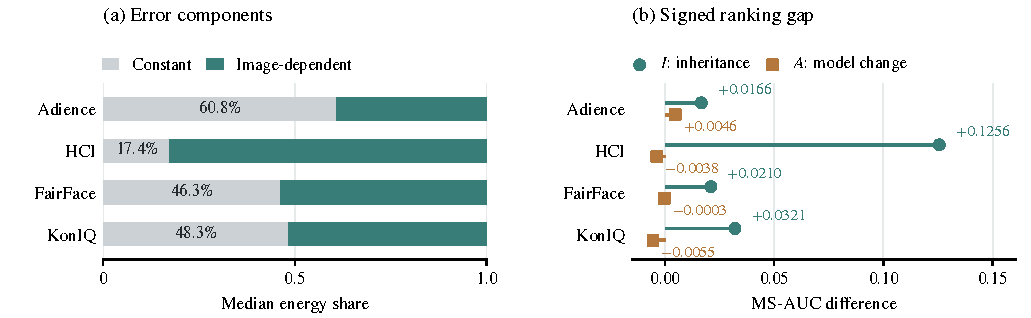
\includegraphics[width=\textwidth]{figures/supp/supp_b_error_diagnostic.pdf}
\caption{\textbf{Inheritance error and the remaining ranking gap.}
(a) Per-dataset median constant-component energy fraction $\kappa$; the complement is the image-dependent share.
(b) Mean signed MS-AUC differences $I$ and $A$ from Eq.~\eqref{eq:supp_fullsupport_gaps}, over the six missing-grade patterns and three seeds, equally averaged over nine adapter configurations.
Negative values indicate that the second score construction ranks better.
These are point summaries; a missing endpoint paired with its nearest seen anchor contributes $A=0$ by construction.}
\label{fig:supp_error_diagnostic}
\end{figure*}

To examine inheritance itself, we use the budget-matched full-support reference, FullSup.
Its displacement is $D^{\mathrm{FS}}=S^{\mathrm{FS}}-T$.
Applying the same inheritance rule gives the diagnostic scores $S^{\mathrm{FS\text{-}TIE}}=T+\mathcal L_{\mathcal U}(D^{\mathrm{FS}})$, denoted FS--TIE.
Define $e_m=D_m^{\mathrm{FS}}-[\mathcal L_{\mathcal U}(D^{\mathrm{FS}})]_m$.
The FullSup and FS--TIE margins against any seen grade differ by exactly $e_m$.
For an isolated interior grade, Proposition~4 of the main paper gives
$e_m=-\tfrac12(D_{m-1}^{\mathrm{FS}}-2D_m^{\mathrm{FS}}+D_{m+1}^{\mathrm{FS}})$.
The error is therefore proportional to the local curvature of adaptation along the grade axis.
Within an interior missing block, equal-weight error also contains a term from the grade's offset from the anchor midpoint; distance weights interpolate linear displacement exactly.

\noindent\textbf{Which part of the error can change the order?}
For a fixed missing--seen pair $(m,n)$, let $\mathbb E_{mn}$ average over test images whose true grades are $m$ or $n$.
We split the error into its mean $c_{mn}=\mathbb E_{mn}[e_m]$ and centered residual $r_{mn}(x)=e_m(x)-c_{mn}$:
\begin{equation}
\begin{aligned}
\mathbb E_{mn}[e_m^2]
&=c_{mn}^2+\mathbb E_{mn}[r_{mn}^2],\\
\kappa_{mn}
&=\frac{c_{mn}^2}{\mathbb E_{mn}[e_m^2]}.
\end{aligned}
\label{eq:supp_error_components}
\end{equation}
Here $\kappa_{mn}$ is the constant-component energy fraction for nonzero error.
For any two images, $e_m(x)-e_m(x')=r_{mn}(x)-r_{mn}(x')$: the constant cancels.
Only the image-dependent component can reorder images.
The diagnostic mean $c_{mn}$ describes this decomposition; it is separate from the validation-selected calibration offset $c^*$.

Figure~\ref{fig:supp_error_diagnostic}a quantifies the distinction.
The median constant-error share ranges from 17\% to 61\% across datasets.
A substantial part of displacement reconstruction error therefore leaves ranking unchanged.
The remaining residual can improve or worsen ranking according to how it changes pair margins.
Reconstruction error alone cannot determine the direction of the ranking change.

\noindent\textbf{Separating inheritance from changes in the adapted model.}
Let $R(Z)$ denote MS-AUC computed from scores $Z$ on the same test images and missing--seen pairs.
With $S^{\mathrm{TIE}}$ from the missing-grade adaptation run, define
\begin{equation}
\begin{aligned}
I
&=R(S^{\mathrm{FS}})
 -R(S^{\mathrm{FS\text{-}TIE}}),\\
A
&=R(S^{\mathrm{FS\text{-}TIE}})
 -R(S^{\mathrm{TIE}}).
\end{aligned}
\label{eq:supp_fullsupport_gaps}
\end{equation}
The total FullSup--TIE gap is exactly $I+A$.
The first term changes only the inherited coordinates within the FullSup model.
The second captures the change in anchors and seen scores between full-support and missing-grade adaptation.
Figure~\ref{fig:supp_error_diagnostic}b reports both signed terms.
For a missing endpoint and its nearest seen anchor, both inherited constructions recover the same zero-shot margin, forcing $A=0$.
Across dataset means, the inheritance term is larger in magnitude than the model-change term.
On HCI, the two terms are 0.126 and $-0.004$, respectively: most of the remaining mean FullSup--TIE gap lies in inheritance within the full-support model.
Proposition~4 characterizes this error, and Proposition~1 identifies the component that can change ranking.
